% B.Tech project report, NIT Warangal.
% Layout follows "Guidelines for Preparation of B.Tech Report" (section numbers in comments).
% Compiles on Overleaf with pdfLaTeX + BibTeX. Figures and numbers in figures/ and
% generated/ are copied in by scripts/make_paper_figures.py; do not edit them by hand.
\documentclass[12pt,a4paper,oneside,openany]{report}

% 2.1.2-2.1.4: A4, Times 12 pt, 1.5 spacing, text 160 x 245 mm, no running header.
\usepackage[a4paper,left=30mm,right=20mm,top=30mm,bottom=22mm,footskip=13mm]{geometry}
\usepackage{amsmath}
\usepackage[T1]{fontenc}
\usepackage{newtxtext,newtxmath} % Times text and maths; provides the AMS symbols
\usepackage{setspace}
\onehalfspacing

\usepackage{graphicx}
\graphicspath{{figures/}}
\usepackage{booktabs,tabularx,array,longtable}
\usepackage{xcolor}
\usepackage{tikz}
\usetikzlibrary{positioning,arrows.meta}
\usepackage[labelfont=bf]{caption}
\usepackage{enumitem}
\usepackage{titlesec}
\usepackage{tocloft}
\usepackage[nottoc]{tocbibind}
\usepackage{cite}
\usepackage[hidelinks]{hyperref}

% ---------------------------------------------------------------------------
% Fill in these details once; every specimen page and header reads them.
% ---------------------------------------------------------------------------
\newcommand{\ProjectTitle}{Byzantine-Resilient Federated Learning for Tactical UAV Swarms over Lossy Wireless Links}

% Students: name and roll number. Add or remove \Student lines as needed.
\newcommand{\StudentList}{%
  \Student{Student Name One}{Roll No. 00XXXXX}%
  \Student{Student Name Two}{Roll No. 00XXXXX}%
  \Student{Student Name Three}{Roll No. 00XXXXX}%
}

\newcommand{\Supervisor}{Dr.~Supervisor Name}
\newcommand{\SupervisorDesignation}{Assistant Professor}
\newcommand{\HOD}{Prof.~HOD Name}
\newcommand{\Department}{Department of Electronics and Communication Engineering}
\newcommand{\Program}{Electronics and Communication Engineering}
\newcommand{\Degree}{Bachelor of Technology}
\newcommand{\SubmissionYear}{2026}
\newcommand{\AcademicYear}{2026--2027}
\newcommand{\Place}{Warangal}
\newcommand{\Phase}{Phase~I (first semester)}

% Generated by scripts/make_paper_figures.py -- do not edit by hand.
\newcommand{\NumRuns}{720}
\newcommand{\NumSeeds}{10}
\newcommand{\PdrTrace}{99.8}
\newcommand{\PdrStress}{65.0}
\newcommand{\TelGain}{-3.5}
\newcommand{\TelLo}{-5.1}
\newcommand{\TelHi}{-2.1}
\newcommand{\MaskGain}{4.2}
\newcommand{\MaskLo}{2.2}
\newcommand{\MaskHi}{5.9}
\newcommand{\PrimGain}{-2.7}
\newcommand{\PrimLo}{-3.9}
\newcommand{\PrimHi}{-1.5}
\newcommand{\AccCcraStress}{46.0}
\newcommand{\AccMaskStress}{49.5}
\newcommand{\AccNoctxStress}{45.3}
\newcommand{\AccFltrustStress}{50.1}
\newcommand{\RejCcra}{41.2}
\newcommand{\RejMask}{13.8}
\newcommand{\AccptCcra}{8.8}
\newcommand{\AccptMask}{13.5}
\newcommand{\RejFltrust}{4.8}
\newcommand{\VsFltTrace}{2.6}
\newcommand{\VsFltTraceLo}{0.9}
\newcommand{\VsFltTraceHi}{4.5}
\newcommand{\VsFltStress}{-0.6}
\newcommand{\VsFltStressLo}{-2.0}
\newcommand{\VsFltStressHi}{1.0}
\newcommand{\DivFedavg}{41}
\newcommand{\DivMedian}{26}
\newcommand{\AllMask}{52.8}
\newcommand{\AllFedavg}{37.3}


% 2.1.7: paragraphs indented 12 mm. The guideline asks for generous separation;
% \ParGap is the one knob to match the department's sample report.
\newlength{\ParGap}\setlength{\ParGap}{6pt}
\setlength{\parindent}{12mm}
\setlength{\parskip}{\ParGap}

% 2.2.1: chapter starts ~75 mm down, "Chapter N" and title centred, 18 pt bold,
% 25 mm between number, title and first paragraph.
\titleformat{\chapter}[display]
  {\centering\bfseries\fontsize{18}{22}\selectfont}
  {\chaptertitlename\ \thechapter}{25mm}{}
\newlength{\ChapterTop}\setlength{\ChapterTop}{75mm}  % extra space above "Chapter N"
\titlespacing*{\chapter}{0pt}{\ChapterTop}{25mm}
% 2.2.2: section 16 pt, subsection 14 pt, bold, flush left, 15 mm around.
\newlength{\SecGap}\setlength{\SecGap}{15mm}
\titleformat{\section}{\bfseries\fontsize{16}{19}\selectfont}{\thesection}{1em}{}
\titlespacing*{\section}{0pt}{\SecGap}{\SecGap}
\titleformat{\subsection}{\bfseries\fontsize{14}{17}\selectfont}{\thesubsection}{1em}{}
\titlespacing*{\subsection}{0pt}{\SecGap}{\SecGap}
% Further subdivisions: unnumbered, not in contents.
\setcounter{secnumdepth}{2}
\setcounter{tocdepth}{2}
\titleformat{\subsubsection}{\bfseries\itshape\normalsize}{}{0pt}{}
\titlespacing*{\subsubsection}{0pt}{3ex}{1ex}

% 3.8: contents with page numbers flushed right.
\renewcommand{\cftchapleader}{\cftdotfill{\cftdotsep}}
\renewcommand{\contentsname}{Contents}

% Numbers used in prose.
\newcommand{\pp}{\,pp}
\newcommand{\ci}[2]{$[#1,\,#2]$}
\newcommand{\Student}[2]{#1 & #2 \\}

\begin{document}

% ---------------------------------------------------------------- front matter
\pagenumbering{roman}
% Specimen A: title sheet (first printed page, no page number).
\begin{titlepage}
\centering
\onehalfspacing
{\fontsize{20}{26}\selectfont\bfseries \ProjectTitle\par}
\vspace{18mm}
{\large Submitted in partial fulfilment of the requirements of the degree of\par}
\vspace{6mm}
{\Large\bfseries \Degree\par}
\vspace{4mm}
{\large in \Program\par}
\vspace{10mm}
{\large by\par}
\vspace{6mm}
{\large
\begin{tabular}{l@{\hspace{12mm}}l}
\StudentList
\end{tabular}\par}
\vspace{12mm}
{\large Supervisor:\par}
\vspace{2mm}
{\large\bfseries \Supervisor\par}
{\large \SupervisorDesignation\par}
\vfill
\IfFileExists{figures/nitw_logo.png}{\includegraphics[width=40mm]{nitw_logo.png}\par\vspace{8mm}}{}
{\large \Department\par}
\vspace{2mm}
{\Large\bfseries NATIONAL INSTITUTE OF TECHNOLOGY WARANGAL\par}
\vspace{4mm}
{\large \SubmissionYear\par}
\end{titlepage}

% Specimen B: approval sheet. First auxiliary page (no dedication), so it is
% page i but shows no number (guidelines 3.6, 3.9).
\clearpage
\setcounter{page}{1}
\thispagestyle{empty}
\begin{center}
{\Large\bfseries Approval for B.Tech Project Report\par}
\end{center}
\vspace{12mm}

{\sloppy
\noindent This Project Work entitled \textbf{``\ProjectTitle''} by
{\renewcommand{\Student}[2]{\StudentSep#1 (#2)\def\StudentSep{, }}\def\StudentSep{}\StudentList}
is approved for the degree of \Degree{} in \Program.\par}

\vspace{25mm}
\noindent
\begin{tabularx}{\textwidth}{@{}X X@{}}
\textbf{Examiners} & \textbf{Supervisor} \\[18mm]
\rule{55mm}{0.4pt} & \rule{55mm}{0.4pt} \\
 & \Supervisor \\[14mm]
\rule{55mm}{0.4pt} & \textbf{Chairman} \\[18mm]
 & \rule{55mm}{0.4pt} \\
\end{tabularx}

\vspace{20mm}
\noindent Date: \rule{40mm}{0.4pt}\par
\noindent Place: \Place

% Specimen C: declaration of academic honesty and integrity (wording prescribed by the institute).
\clearpage
\begin{center}
{\Large\bfseries Declaration\par}
\end{center}
\vspace{8mm}

I declare that this written submission represents my ideas in my own words and where
others' ideas or words have been included, I have adequately cited and referenced the
original sources. I also declare that I have adhered to all principles of academic
honesty and integrity and have not misrepresented or fabricated or falsified any
idea/data/fact/source in my submission. I understand that any violation of the above
will be cause for disciplinary action by the Institute and can also evoke penal action
from the sources which have thus not been properly cited or from whom proper permission
has not been taken when needed.

\vspace{18mm}
\noindent
{\renewcommand{\Student}[2]{%
  \begin{minipage}[t]{0.32\textwidth}\centering
  \rule{40mm}{0.4pt}\\(Signature)\\#1\\#2
  \end{minipage}\hfill}%
\StudentList}

\vspace{14mm}
\noindent Date: \rule{40mm}{0.4pt}

% Specimen D: certificate.
\clearpage
\begin{center}
{\large\bfseries \Department\par}
{\large\bfseries National Institute of Technology Warangal\par}
\vspace{10mm}
{\Large\bfseries Certificate\par}
\end{center}
\vspace{8mm}

This is to certify that the Project work entitled \textbf{``\ProjectTitle''} is a
bonafide record of work carried out by
{\renewcommand{\Student}[2]{\StudentSep\textbf{#1} (#2)\def\StudentSep{, }}\def\StudentSep{}\StudentList},
submitted to the faculty of the \Department, in partial fulfilment of the requirements
for the award of the degree of \Degree{} in \Program{} at National Institute of
Technology, Warangal during the academic year \AcademicYear.

\vspace{30mm}
\noindent
\begin{tabularx}{\textwidth}{@{}X X@{}}
\rule{55mm}{0.4pt} & \rule{55mm}{0.4pt} \\
\HOD & \Supervisor \\
Head of the Department & \SupervisorDesignation \\
\Department & \Department \\
\end{tabularx}

% 3.7: abstract, at most 500 words.
\chapter*{Abstract}
\addcontentsline{toc}{chapter}{Abstract}

Swarms of unmanned aerial vehicles (UAVs) can learn a shared perception model with
federated learning (FL): each UAV trains on the images it collects and sends only a
model update to a ground base station. In a tactical setting two problems arise
together. Air-to-ground links lose packets because of fading, distance, handover and
jamming, and some UAVs may be captured and made to send poisoned updates. Most
Byzantine-robust aggregation rules assume that every update arrives intact, while
most work on FL over unreliable links assumes that every client is honest. This
project studies both problems in one system.

We built a simulation framework in PyTorch for hierarchical FL over a UAV swarm. Ten
UAVs with non-identically distributed aerial images are served by three base
stations, which aggregate locally and synchronize every five rounds. Uplink packet
losses come either from a synthetic channel with path loss, Rayleigh fading and a
ground jammer, or from a measured UAV received-power trace (DeepSense~6G Scenario~23)
replayed at a chosen signal-to-noise ratio. Three of the UAVs mount sign-flip,
ALIE-style or inner-product-manipulation attacks. The framework includes FedAvg,
coordinate-wise median, FLTrust, a cosine-weighted rule taken from prior UAV-FL
work, and a reputation-based aggregator, CCRA, that we designed. CCRA compares each
update with a reference update computed on a small trusted dataset, keeps a
reputation for every UAV across rounds, and can use link information in two ways:
by ignoring coordinates whose packets were lost (erasure masking), and by letting
link telemetry slow down how fast a UAV regains trust.

The work proceeded in three phases. A FedAvg baseline reached
62.6\% (IID) and 60.2\% (non-IID) test accuracy. A preliminary single-seed study
suggested that CCRA resisted a label-flipping attack better than the cosine-weighted
baseline. To test which part of CCRA was responsible, we then ran a controlled,
prespecified study of \NumRuns{} training runs on an A100 GPU: \NumSeeds{} paired
seeds, four attack settings, three channel conditions and six aggregators. Diverged
runs were scored at chance rather than discarded, and all uncertainty was estimated
with a paired bootstrap over seeds.

The study gave a clear and partly negative answer. On a weak (5\,dB) link under
attack, erasure masking improved accuracy by \MaskGain{} percentage points (95\%
confidence interval \ci{\MaskLo}{\MaskHi}). Adding link telemetry to the reputation
update changed accuracy by \TelGain{} points (\ci{\TelLo}{\TelHi}) because it
rejected \RejCcra\% of honest updates, against \RejMask\% without telemetry. We
explain this with a short analysis of the reputation rule: when rewards are slowed
but penalties are not, an honest UAV's reputation settles near its worst rounds. All
reference-based aggregators avoided divergence, whereas FedAvg and the median
diverged in \DivFedavg{} and \DivMedian{} of 120 runs.

The result changes the direction of the project. The useful channel-aware component
is erasure masking, and the reputation reward rule must be redesigned before link
telemetry can help. The findings are written up as a four-page letter in IEEE format.
The second phase will revise the reward rule, test it on fresh seeds and
higher-mobility traces, and evaluate adaptive attackers.

\vspace{6mm}
\noindent\textbf{Keywords:} federated learning, UAV swarm, Byzantine robustness,
packet erasure, hierarchical aggregation, reputation.


\clearpage
\tableofcontents
\clearpage
\listoffigures
\clearpage
\listoftables
% 3.9: abbreviations, notation and nomenclature.
\chapter*{Abbreviations and Notation}
\addcontentsline{toc}{chapter}{Abbreviations and Notation}

\section*{Abbreviations}
\begin{longtable}{@{}p{32mm}p{122mm}@{}}
ALIE & A Little Is Enough (model-poisoning attack) \\
BS & Base station \\
CCRA & Context-Calibrated Robust Aggregation (the aggregator studied here) \\
CI & Confidence interval \\
CNN & Convolutional neural network \\
CosAvg & Cosine-similarity weighted averaging \\
EMA & Exponential moving average \\
EW & Electronic warfare \\
FedAvg & Federated averaging \\
FL & Federated learning \\
HFL & Hierarchical federated learning \\
IID & Independent and identically distributed \\
IPM & Inner-product manipulation (model-poisoning attack) \\
PDR & Packet delivery ratio \\
PER & Packet error rate \\
pp & Percentage points \\
RMS & Root mean square \\
SGD & Stochastic gradient descent \\
SINR & Signal-to-interference-plus-noise ratio \\
SNR & Signal-to-noise ratio \\
TEE & Trusted execution environment \\
UAV & Unmanned aerial vehicle \\
\end{longtable}

\section*{Notation}
\begin{longtable}{@{}p{32mm}p{122mm}@{}}
$K$ & Number of UAVs (clients) \\
$B$ & Number of base stations \\
$E$ & Edge rounds between global synchronizations \\
$P$ & Number of model parameters \\
$L$ & Parameters per packet \\
$f$ & Number of Byzantine UAVs \\
$\mathcal{D}_k$, $n_k$ & Local dataset of UAV $k$ and its size \\
$\mathcal{D}_0$ & Trusted root dataset held by each base station \\
$\mathbf{w}^t$, $\mathbf{w}^t_b$ & Global model and edge model of BS $b$ in round $t$ \\
$\boldsymbol{\Delta}_k^t$ & Model update sent by UAV $k$ in round $t$ \\
$\mathbf{m}_k$ & Delivery mask: 1 where the packet carrying a coordinate arrived \\
$\mathbf{r}$ & Reference update computed on $\mathcal{D}_0$ \\
$\gamma_k$, $\bar\gamma$ & Uplink SNR of UAV $k$; reference SNR of the trace \\
$p_k$ & Packet error probability of UAV $k$ \\
$a$, $\gamma_{\mathrm{th}}$ & Slope and threshold of the packet-error curve \\
$s_k$ & Norm-clipping factor \\
$c_k$ & Masked cosine similarity to the reference update \\
$b_k$ & Behaviour score in $[0,1]$ \\
$T_k$ & Reputation (trust) of UAV $k$ \\
$e_k$ & Link evidence in $[0,1]$ that slows reputation rewards \\
$\beta$, $\tau$ & Reputation memory and exclusion gate \\
$\omega_k$ & Aggregation weight of UAV $k$ \\
$\alpha$ & Dirichlet concentration of the non-IID data split \\
$\lambda$, $z$, $\epsilon$ & Strengths of the sign-flip, ALIE and IPM attacks \\
\end{longtable}


% ---------------------------------------------------------------- main text
\clearpage
\pagenumbering{arabic}
\chapter{Introduction}
\thispagestyle{empty} % 2.1.5: page 1 of the Introduction bears no number.
\label{ch:intro}

\section{Background}
Small unmanned aerial vehicles (UAVs) are now used in groups, or swarms, for
surveillance, search and rescue, disaster assessment and border patrol. Each UAV
carries a camera and collects images of the area it covers. A perception model
trained on all of these images is more accurate than one trained on any single
UAV's data, but sending raw imagery to a ground station is costly in bandwidth and
exposes sensitive data if a link is intercepted.

Federated learning (FL) addresses this by moving training to the data. Each UAV
trains a copy of the model on its own images and uploads only the resulting model
update. A server (here, a ground base station) combines the updates into a new
global model and sends it back. The raw images never leave the UAV, and an update is
usually much smaller than the data it was computed from.

A tactical swarm, however, breaks two assumptions that standard FL relies on.
\begin{enumerate}
\item \textbf{Links are unreliable.} Air-to-ground channels fade as the UAV moves,
  hand over between base stations, and may be deliberately jammed. Parts of an update
  are lost, and some updates miss the round deadline entirely.
\item \textbf{Some clients may be hostile.} A captured or spoofed UAV can follow the
  protocol while sending a poisoned update designed to damage the global model. Such
  clients are called \emph{Byzantine}.
\end{enumerate}
Most Byzantine-robust aggregation rules assume that every update arrives intact, and
most work on FL over imperfect channels assumes that every client is honest. A swarm
needs both at once.

\section{Problem Statement}
Given a UAV swarm that trains a shared image classifier with hierarchical FL over
lossy air-to-ground links, in which a minority of UAVs are Byzantine, design and
evaluate an aggregation rule that (i) keeps the global model accurate and stable,
(ii) does not penalize honest UAVs simply because their links are poor, and
(iii) can be compared fairly against established rules under identical conditions.

\section{Aim and Scope}
The aim of this project is to determine \emph{which} kind of channel awareness
actually helps a robust aggregator in a UAV swarm, and to quantify the effect with a
controlled, reproducible experiment. Its scope in Phase~I is:
\begin{itemize}
\item a simulation of hierarchical FL with up to three base stations, UAV
  association and handover;
\item packet-level uplink losses from a synthetic jammed channel and from a measured
  UAV received-power trace;
\item four model-poisoning and data-poisoning attacks;
\item six aggregation rules evaluated on the same data, models, attackers and channel
  realizations.
\end{itemize}
Hardware flight tests, real radio transmission and attacks that forge link telemetry
are outside the Phase~I scope.

\section{Objectives}
\begin{enumerate}
\item Build an FL baseline for a UAV swarm on an aerial image dataset and measure its
  accuracy under IID and non-IID data.
\item Model a lossy uplink in which lost packets erase parts of an update, and add
  Byzantine attackers.
\item Design a reputation-based aggregator (CCRA) that uses a trusted reference
  update, and give it two forms of channel awareness: erasure masking and
  telemetry-weighted reputation.
\item Separate the effect of each component with a prespecified, multi-seed ablation
  study, and report the results with honest uncertainty estimates.
\end{enumerate}

\section{Contributions}
\begin{itemize}
\item An open, tested PyTorch framework for hierarchical UAV-swarm FL with
  trace-driven packet erasures, handover and five attacks (43 automated tests).
\item A preliminary study, then a controlled \NumRuns-run study whose analysis plan
  and decision threshold were fixed before the runs.
\item The finding that erasure masking improves accuracy under attack on weak links
  by \MaskGain{} percentage points, while telemetry-weighted reputation lowers it,
  together with an analysis of the reputation rule that explains why.
\item A four-page manuscript in IEEE letter format that reports these results.
\end{itemize}

\section{Organization of the Report}
Chapter~\ref{ch:lit} reviews federated learning, Byzantine-robust aggregation and FL
over unreliable wireless links, and identifies the gap this project addresses.
Chapter~\ref{ch:method} describes the system model, the threat model, the
aggregation rules and the experimental protocol. Chapter~\ref{ch:results} presents
the baseline, the preliminary study and the controlled study, and discusses what
they show. Chapter~\ref{ch:conclusions} summarizes the conclusions and the plan for
Phase~II. The appendices list the hyperparameters and the steps needed to reproduce
every result.

\chapter{Review of Literature}
\label{ch:lit}

\section{Federated Learning}
McMahan \textit{et al.}~\cite{mcmahan2017fedavg} introduced federated averaging
(FedAvg). In each round the server sends the global model to a set of clients, each
client runs a few epochs of stochastic gradient descent on its local data, and the
server replaces the global model by the average of the returned models, weighted by
local dataset size. FedAvg works well when client data are independent and
identically distributed (IID). When each client sees a skewed mix of classes, local
models drift apart and accuracy falls. Hsu \textit{et al.}~\cite{hsu2019noniid}
proposed sampling each client's class proportions from a Dirichlet distribution with
concentration $\alpha$, which has become the standard way to control the degree of
non-IID skew in experiments; we use $\alpha=0.5$.

Hierarchical FL adds an intermediate layer of edge servers. Clients send updates to a
nearby edge server, which aggregates them frequently, and the edge servers
synchronize with each other less often. This matches a UAV swarm served by several
ground base stations, each covering part of the operating area.

\section{Byzantine-Robust Aggregation}
A single malicious client can move the FedAvg average arbitrarily far, so a large
body of work replaces the mean by a robust statistic.
\begin{itemize}
\item \textbf{Krum}~\cite{blanchard2017krum} selects the update whose summed distance
  to its nearest neighbours is smallest. It requires $n\ge 2f+3$ clients to tolerate
  $f$ attackers.
\item \textbf{Coordinate-wise median and trimmed mean}~\cite{yin2018median} take the
  median, or a trimmed mean, of each parameter separately, and come with statistical
  error guarantees.
\item \textbf{FLTrust}~\cite{cao2021fltrust} gives the server a small clean root
  dataset. The server computes its own update on that data each round, scores each
  client by the (clipped at zero) cosine similarity to it, and rescales every client
  update to the norm of the server update before averaging.
\end{itemize}
These rules are evaluated against attacks of increasing strength. A sign-flip attack
sends a scaled negative of an honest update. ALIE (``A Little Is Enough'')
\cite{baruch2019alie} shifts each coordinate by a small multiple of the honest
standard deviation, which is enough to evade distance-based rules. Inner-product
manipulation (IPM)~\cite{xie2019ipm} sends a negative multiple of the honest mean so
that the aggregate's inner product with the true gradient becomes negative.

Reputation-based defences keep a trust score for each client across rounds, so that
an attacker caught once stays down-weighted. They suit swarms, whose members persist
for a whole mission, but recent work shows that adaptive attackers can learn to evade
them~\cite{liu2026evade}.

\section{Federated Learning over Unreliable Wireless Links}
In wireless FL the update itself travels over a noisy channel. Shirvanimoghaddam
\textit{et al.}~\cite{shirvanimoghaddam2022erroneous} study FL in which the
communication links are erroneous; this letter is the base paper for our study of
lossy links. Barkatsa \textit{et al.}~\cite{barkatsa2024jamming} address jamming
attacks on wireless FL networks with a Bayesian-game formulation. Li
\textit{et al.}~\cite{li2022dpbyz} combine communication efficiency, differential
privacy and Byzantine robustness. In each case the emphasis is on either the channel
or the adversary, not on how lost packets interact with a robust aggregator.

\section{Federated Learning for UAV Swarms}
Xiao \textit{et al.}~\cite{xiao2021uavswarm} propose fully decentralized FL for
on-board missions of a UAV swarm. Liao \textit{et al.}~\cite{liao2023tee} propose
UAV-assisted FL based on a trusted execution environment (TEE) and aggregate updates
by their cosine similarity to the mean update (CosAvg); our preliminary study
re-implements CosAvg as a baseline. Realistic UAV link data have recently become
available: the DeepSense~6G dataset~\cite{alkhateeb2023deepsense} includes a
scenario with a flying UAV and a ground base station~\cite{charan2025drone}, which we
use to drive packet losses in simulation.

\section{Research Gap}
Table~\ref{tab:gap} summarizes the gap. Robust rules either compare updates as if
they were complete, treating a lost packet as a zero, or ignore the channel entirely.
Channel-aware designs do not model adversarial clients. It is also natural to assume
that link telemetry (signal quality, delivery ratio, handover state) should make a
robust aggregator \emph{fairer} to honest UAVs on poor links, but we found no
controlled test of that assumption. This project provides one.

\begin{table}[ht]
\centering
\caption[Coverage of the problem in the reviewed work]{Coverage of the problem in the
reviewed work. Entries for the letters~\cite{shirvanimoghaddam2022erroneous,barkatsa2024jamming,xiao2021uavswarm}
and for~\cite{liao2023tee} reflect their titles and our reading so far and are to be
confirmed against the full texts.}
\label{tab:gap}
\small
\begin{tabularx}{\textwidth}{@{}X c c c c@{}}
\toprule
Work & Byzantine clients & Packet loss & UAV setting & Measured channel \\
\midrule
FedAvg~\cite{mcmahan2017fedavg} & -- & -- & -- & -- \\
Krum, median~\cite{blanchard2017krum,yin2018median} & \checkmark & -- & -- & -- \\
FLTrust~\cite{cao2021fltrust} & \checkmark & -- & -- & -- \\
Erroneous links~\cite{shirvanimoghaddam2022erroneous} & -- & \checkmark & -- & -- \\
Jamming mitigation~\cite{barkatsa2024jamming} & -- & \checkmark & -- & -- \\
UAV-swarm FL~\cite{xiao2021uavswarm} & -- & -- & \checkmark & -- \\
TEE + CosAvg~\cite{liao2023tee} & \checkmark & -- & \checkmark & -- \\
\textbf{This project} & \checkmark & \checkmark & \checkmark & \checkmark \\
\bottomrule
\end{tabularx}
\end{table}

\chapter{System Model and Methodology}
\label{ch:method}

This chapter describes the simulated system, the attacker, the aggregation rules
compared, and the protocol used to evaluate them. All of it is implemented in the
project repository; file names are given where they help locate the code.

\section{Hierarchical Federated Learning for a UAV Swarm}

\begin{figure}[ht]
\centering
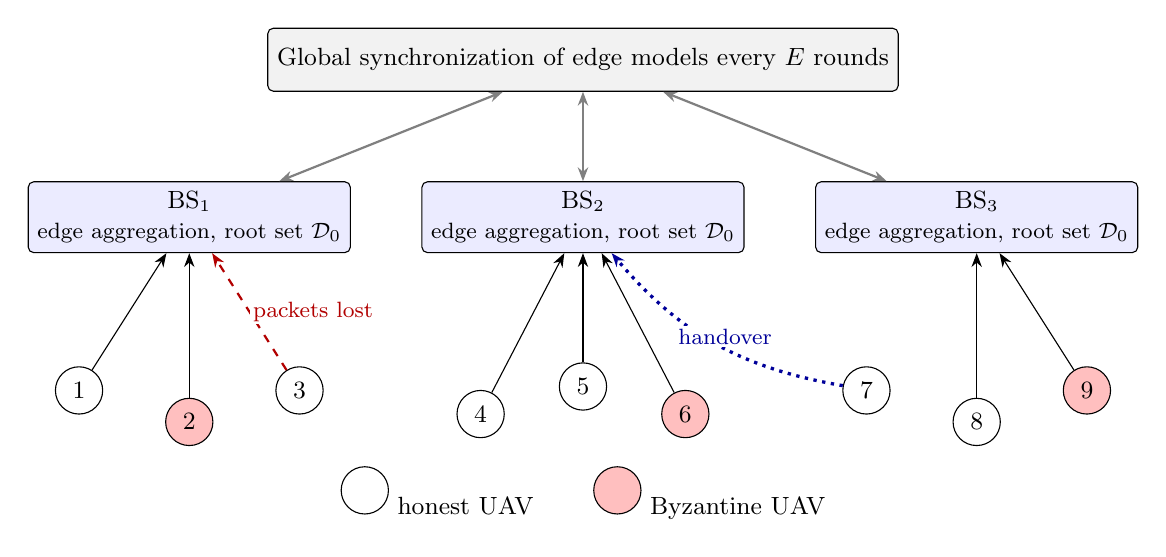
\begin{tikzpicture}[
  font=\small, >={Stealth[length=5pt]},
  bs/.style={draw, fill=blue!8, rounded corners=2pt, minimum width=20mm, minimum height=9mm, align=center},
  uav/.style={circle, draw, fill=white, inner sep=0pt, minimum size=6mm},
  bad/.style={uav, fill=red!25},
  cloud/.style={draw, fill=gray!10, rounded corners=2pt, minimum width=70mm, minimum height=8mm, align=center}]
  \node[cloud] (g) at (0,4.2) {Global synchronization of edge models every $E$ rounds};
  \foreach \x/\n in {-5/1,0/2,5/3} {
    \node[bs] (b\n) at (\x,2.2) {BS$_\n$\\{\footnotesize edge aggregation, root set $\mathcal{D}_0$}};
    \draw[<->, gray, thick] (b\n) -- (g);
  }
  \node[uav] (u1) at (-6.4,0) {1};  \node[bad] (u2) at (-5,-0.4) {2};  \node[uav] (u3) at (-3.6,0) {3};
  \node[uav] (u4) at (-1.3,-0.3) {4}; \node[uav] (u5) at (0,0.05) {5};  \node[bad] (u6) at (1.3,-0.3) {6};
  \node[uav] (u7) at (3.6,0) {7};   \node[uav] (u8) at (5,-0.4) {8};   \node[bad] (u9) at (6.4,0) {9};
  \foreach \u/\b in {1/1,2/1,4/2,5/2,6/2,8/3,9/3} \draw[->] (u\u) -- (b\b);
  \draw[->, dashed, red!70!black, thick] (u3) -- node[pos=0.5, right, fill=white, inner sep=1pt] {\footnotesize packets lost} (b1);
  \draw[->, dotted, very thick, blue!60!black] (u7) to[bend left=20] node[pos=0.45, above, fill=white, inner sep=1pt] {\footnotesize handover} (b2);
  \node at (0,-1.3) {\tikz\node[uav]{};~honest UAV \qquad \tikz\node[bad]{};~Byzantine UAV};
\end{tikzpicture}
\caption{Hierarchical FL over a UAV swarm. Each base station aggregates the updates of
the UAVs it serves, some of which arrive with lost packets; edge models are
synchronized every $E$ rounds.}
\label{fig:system}
\end{figure}

Figure~\ref{fig:system} shows the system. $K$ UAVs are served by $B$ ground base
stations (BSs). Each UAV $k$ holds a private dataset $\mathcal{D}_k$ of $n_k$ images.
In every round $t$:
\begin{enumerate}
\item each UAV attached to BS $b$ starts from that BS's edge model $\mathbf{w}^t_b$
  and trains it for one local epoch of SGD on $\mathcal{D}_k$;
\item it uploads the update $\boldsymbol{\Delta}^t_k$ (new local model minus the edge
  model), which is split into packets of $L$ parameters;
\item the BS aggregates the updates it receives and sets
  $\mathbf{w}^{t+1}_b=\mathbf{w}^t_b+\mathrm{Agg}(\cdot)$;
\item every $E$ rounds the edge models are averaged, weighted by the number of
  training samples held by the UAVs in each cell, and the result is sent back to
  every BS.
\end{enumerate}
UAVs attach to the BS with the strongest received power. A UAV hands over only when
another BS is stronger by a hysteresis margin of 3\,dB for two consecutive rounds,
which avoids ping-pong handovers (\texttt{fl/topology.py}).

\subsection{Dataset and Model}
Images come from CIFAR-10, modified to resemble aerial imagery
(\texttt{fl/data.py}). Each image is rotated by a random multiple of
$90^\circ$, since a downward-looking camera has no preferred orientation, and with
probability 0.3 or 0.2 is down-sampled to $24\times24$ or $16\times16$ pixels and
up-sampled again to imitate higher flight altitudes. The 50{,}000 training images
are split among the UAVs either uniformly (IID) or with Dirichlet($\alpha$)
class proportions; 500 images (50 per class) are held out as the trusted root set
$\mathcal{D}_0$ and are never given to any UAV.

The classifier, TacticalEdgeCNN, is a small convolutional network with about 156k
parameters and group normalization, chosen so that it could plausibly be trained on
board. Group normalization is used instead of batch normalization because batch
statistics do not average well across clients with different class mixes.

\section{Wireless Uplink Models}
\label{sec:channel}
The channel decides, for every packet of every update, whether it arrives
(\texttt{fl/channel.py}). Two models are used.

\subsection{Synthetic Jammed Channel}
UAVs move by a random walk at 100\,m altitude over an $800\times800$\,m area. The
received power from UAV $k$ at its serving BS is
\begin{equation}
  P_{\mathrm{rx},k} = P_{\mathrm{tx}} - \mathrm{PL}(d_k) + 10\log_{10}|h_k|^2,
  \qquad \mathrm{PL}(d)=40+10\eta\log_{10}d \ \text{dB},
\end{equation}
with $P_{\mathrm{tx}}=20$\,dBm, path-loss exponent $\eta=2.2$, and Rayleigh fading
$|h_k|^2\sim\mathrm{Exp}(1)$. A ground jammer of power 10\,dBm targets a sector of
the swarm, and the SINR is
\begin{equation}
  \gamma_k = P_{\mathrm{rx},k} - 10\log_{10}\bigl(N_0 + J_k\bigr),
\end{equation}
where $N_0$ corresponds to $-90$\,dBm and $J_k$ is the jamming power received at
UAV $k$'s link (zero for UAVs outside the jammed sector).

\subsection{Measured-Trace Channel}
For realism we replay a measured UAV link from DeepSense~6G
Scenario~23~\cite{alkhateeb2023deepsense,charan2025drone}, in which a drone flies
around a ground receiver that records 60\,GHz beam powers together with position,
altitude and speed. The dataset's power values are uncalibrated, so only their
variation relative to the median is used:
\begin{equation}
  \gamma_k = \bar\gamma + \bigl(P^{\mathrm{meas}}_k - \mathrm{med}\,P^{\mathrm{meas}}\bigr)
  - 10\eta\log_{10}\frac{d_{k,b}}{d_{k,1}},
\end{equation}
where $\bar\gamma$ is an assumed reference SNR and the last term adjusts the measured
link to the distance of a virtual BS $b$. Each UAV replays a different flight
segment. Two settings are used: $\bar\gamma=15$\,dB, a good link, and
$\bar\gamma=5$\,dB, a weak link. They replay identical trajectories, so only the
link quality differs.

\subsection{Packet Erasures}
In both models each packet is lost independently with probability
\begin{equation}
  p_k = \frac{1}{1+\exp\bigl(a(\gamma_k-\gamma_{\mathrm{th}})\bigr)},
\end{equation}
with $a=1$ and $\gamma_{\mathrm{th}}=3$\,dB. An update whose transmission time at
the Shannon rate exceeds the 2\,s round deadline is dropped entirely. The BS
therefore receives $\tilde{\boldsymbol\Delta}_k=\mathbf{m}_k\odot\boldsymbol\Delta_k$,
where the mask $\mathbf{m}_k$ is 1 for delivered coordinates and 0 elsewhere. The BS
also records link telemetry for each UAV: SNR, packet delivery ratio (PDR), long-run
reliability, distance, speed and handover state.

\section{Threat Model}
A fixed set of $f=3$ of the $K=10$ UAVs is Byzantine. They follow the protocol (they
train, transmit on time and use the same channel) but replace their update with one
of the following (\texttt{fl/attacks.py}, \texttt{fl/client.py}):
\begin{itemize}
\item \textbf{Label flip} (data poisoning): train on labels mapped $c\mapsto 9-c$.
\item \textbf{Sign flip}: send $-\lambda\boldsymbol\Delta_k$ with $\lambda=5$.
\item \textbf{ALIE-style}~\cite{baruch2019alie}: send
  $\boldsymbol\mu-z\,\boldsymbol\sigma\odot\mathrm{sign}(\boldsymbol\mu)$ with $z=1.5$,
  where $\boldsymbol\mu$ and $\boldsymbol\sigma$ are the mean and standard deviation of
  the honest updates in the attacker's cell.
\item \textbf{IPM}~\cite{xie2019ipm}: send $-\epsilon\boldsymbol\mu$ with $\epsilon=0.5$.
\end{itemize}
The ALIE and IPM attackers know the honest updates of their cell, which is a strong
assumption chosen to stress the defences. The BS's telemetry is assumed authentic;
attacks that forge it are left for Phase~II.

\section{Aggregation Rules}
All rules receive exactly the same inputs: the received updates, their masks, sample
counts and telemetry (\texttt{fl/aggregators.py}).

\subsection{Baselines}
\textbf{FedAvg}~\cite{mcmahan2017fedavg} averages the received updates weighted by
$n_k$, with lost coordinates counted as zeros. \textbf{CosAvg}, the aggregation of the
earlier UAV-FL work~\cite{liao2023tee} as re-implemented here, weights each update by
$\max(0,\cos(\boldsymbol\Delta_k,\bar{\boldsymbol\Delta}))\,n_k$, where
$\bar{\boldsymbol\Delta}$ is the FedAvg mean. \textbf{Coordinate-wise
median}~\cite{yin2018median} takes the median of the delivered values of each
parameter. \textbf{FLTrust}~\cite{cao2021fltrust} computes a root update $\mathbf{r}$
on $\mathcal{D}_0$ (with as many local steps as a typical UAV), weights each UAV by
$\max(0,\cos)$ to $\mathbf{r}$ on delivered coordinates, and rescales each update to
the norm of $\mathbf{r}$.

\subsection{Context-Calibrated Robust Aggregation (CCRA)}
CCRA is the aggregator designed in this project. Each BS applies the following
steps every round.
\begin{enumerate}
\item \textbf{Reference update.} Compute $\mathbf{r}$ on $\mathcal{D}_0$, as in FLTrust.
  Our diagnostics showed that, under non-IID data, the mean or median of the UAV
  updates is not a reliable reference: attackers and honest UAVs with skewed data
  had similar cosine similarity to it.
\item \textbf{Norm clipping.} Let $\rho_k$ be the RMS of the delivered entries of
  $\tilde{\boldsymbol\Delta}_k$ and scale the update by
  $s_k=\min(1,\ \mathrm{med}_j\rho_j/\rho_k)$, which defeats scaling attacks.
\item \textbf{Masked similarity.}
  $c_k=\cos\bigl(\mathcal{S}(s_k\tilde{\boldsymbol\Delta}_k;\mathbf{m}_k),\
  \mathcal{S}(\mathbf{r};\mathbf{m}_k)\bigr)$, where $\mathcal{S}(\cdot;\mathbf{m})$
  keeps only the coordinates with $\mathbf{m}=1$. Lost packets therefore do not make
  an honest update look dissimilar.
\item \textbf{Behaviour score.} $b_k=\mathrm{clip}\bigl(c_k/\mathrm{med}_{j:c_j>0}c_j,\
  0,\ 1\bigr)$. Updates pointing away from the reference get $b_k=0$.
\item \textbf{Reputation.} With memory $\beta$, initial trust 1 and evidence
  $e_k\in[0,1]$,
  \begin{equation}
    T_k \leftarrow T_k+\eta_k(b_k-T_k),\qquad
    \eta_k=\begin{cases}(1-\beta)\,e_k, & b_k>T_k,\\ 1-\beta, & b_k\le T_k.\end{cases}
    \label{eq:reputation}
  \end{equation}
  Penalties apply at full rate, so an attacker cannot hide by dropping its own
  packets; only rewards are slowed on poor links.
\item \textbf{Gating and averaging.} UAVs with $T_k<\tau$ are excluded. The others get
  weight $\omega_k=n_kT_k$, discounted for staleness, and each coordinate is averaged
  only over the UAVs that delivered it:
  \begin{equation}
    \mathrm{Agg}_p=\frac{\sum_k\omega_k\,m_{k,p}\,s_k\tilde\Delta_{k,p}}
                      {\sum_k\omega_k\,m_{k,p}}.
    \label{eq:masked-average}
  \end{equation}
\end{enumerate}
The evidence term multiplies five link factors:
\begin{equation}
  e_k=\mathrm{PDR}_k\cdot R_k\cdot h_k\cdot\frac{1}{1+d_k/A}\cdot\frac{1}{1+|v_k|},
\end{equation}
namely the packet delivery ratio, long-run reliability, a handover factor
($h_k=0.5$ during a handover, 1 otherwise), a distance factor with $A$ the area size,
and a normalized-speed factor.

\subsection{Ablation Variants}
To find out which part of CCRA matters, three variants are compared.
\begin{itemize}
\item \textbf{CCRA (full)}: all steps, with evidence $e_k$ from telemetry.
\item \textbf{Mask-only}: $e_k=1$, but the masks are used in steps 2--6.
\item \textbf{No-context}: $e_k=1$ and $\mathbf{m}_k=\mathbf{1}$, so lost
  coordinates enter the computation as zeros, as a channel-unaware server would see
  them.
\end{itemize}
The code also has an option to correct $c_k$ for the noise expected at the
reported SINR. It is inactive in the controlled study, which adds no residual noise
to delivered parameters, so the full-versus-mask-only contrast isolates $e_k$.

\subsection{Analysis of the Reputation Update}
\label{sec:fixed-point}
The asymmetric update~\eqref{eq:reputation} has a consequence that was not intended.
Suppose a UAV's evidence is constant, $e_k=e$, and its scores $b$ are drawn
independently from some distribution. The expected change in reputation is
\begin{equation}
  \mathbb{E}[\Delta T] = (1-\beta)\Bigl(e\,\mathbb{E}\bigl[(b-T)^+\bigr]
                        - \mathbb{E}\bigl[(T-b)^+\bigr]\Bigr),
\end{equation}
so the reputation settles where
\begin{equation}
  e\,\mathbb{E}\bigl[(b-T^\star)^+\bigr] = \mathbb{E}\bigl[(T^\star-b)^+\bigr].
  \label{eq:fixed-point}
\end{equation}
For $e=1$ the two sides balance at $T^\star=\mathbb{E}[b]$, the mean score. As $e$
decreases, the left side shrinks, and $T^\star$ must move down until few scores lie
below it; in the limit $e\to0$ it approaches the lowest score the UAV ever receives.
An honest UAV with skewed data has noisy scores, so on a weak link its reputation
tracks its worst rounds and falls below the gate $\tau$ more often. An attacker's
scores are already near zero, so slowing its rewards adds little. Section~\ref{sec:mechanism}
tests this prediction against the measured gate decisions.

\section{Implementation and Verification}
The framework is written in Python with PyTorch. Runs are configured by a single
dataclass, and every run stores its full configuration, per-round history and final
model. The repository contains 43 automated tests covering data partitioning, the
FedAvg update, attack construction, every robust aggregator, the hierarchical server,
handover logic, trace loading and the analysis code. A code review of the
hierarchical extension found three problems, which were fixed before the controlled
study was run: the reputation rule shielded jammed attackers, the no-context
ablation still read packet delivery ratios, and FLTrust's root update took too few
training steps.

\section{Experimental Protocol}
\subsection{Preliminary Study}
The first comparison used the synthetic jammed channel with one BS, a 30\% label-flip
attack, 30 rounds and a single seed. It compared FedAvg, CosAvg and an early version
of CCRA under four scenarios: no attack or attack, each with an ideal or a jammed
lossy channel. Its purpose was to check that the pipeline worked and to estimate
effect sizes.

\subsection{Controlled Ablation Study}
\label{sec:protocol}
The main study used a full factorial design: six aggregators (FedAvg, median,
FLTrust and the three CCRA variants), four attack settings (clean, sign flip, ALIE,
IPM), three channel conditions (ideal; trace at 15\,dB; trace at 5\,dB) and
\NumSeeds{} seeds, for \NumRuns{} runs of 100 rounds each with $K=10$, $B=3$, $E=5$
and $\alpha=0.5$. Within a seed, the data split, initial model, attacker identities
and trace positions are identical across methods, so every comparison is paired. The
runs were executed on an NVIDIA A100 GPU.

The analysis plan was fixed before any run:
\begin{itemize}
\item The \emph{primary} quantity is the telemetry effect under stress,
  $[(\text{CCRA}-\text{mask-only})_{5\,\mathrm{dB}}-(\text{CCRA}-\text{mask-only})_{15\,\mathrm{dB}}]$,
  averaged over the three attacks within each seed.
\item An effect counts as practically meaningful only if its 95\% interval lies
  entirely beyond $\pm1$ percentage point.
\item Intervals are percentile bootstraps over seeds with 10{,}000 resamples; rounds
  and attack cells are not treated as independent samples.
\item A run that diverges numerically is scored at chance accuracy (10\%) instead of
  being dropped, so unstable methods cannot look better by losing their worst runs.
\item All other contrasts are exploratory and are not adjusted for multiple
  comparisons.
\end{itemize}

\chapter{Results and Discussion}
\label{ch:results}

The results are presented in the order the work was done: the FedAvg baseline, the
preliminary single-seed study, and the controlled \NumRuns-run study. Every number in
Section~\ref{sec:controlled} is generated from the committed run-level data by the
script described in Appendix~\ref{app:repro}.

\section{FedAvg Baseline}
The first objective was a working FL pipeline without any defence. Ten UAVs trained
TacticalEdgeCNN for 50 rounds with two local epochs, SGD (learning rate 0.01,
momentum 0.9, batch size 64), on one BS with an ideal channel.
Table~\ref{tab:baseline} and Fig.~\ref{fig:baseline} show the result.

\begin{table}[ht]
\centering
\caption{FedAvg baseline accuracy after 50 rounds}
\label{tab:baseline}
\begin{tabular}{@{}lcc@{}}
\toprule
Data partition & Final test accuracy (\%) & Best test accuracy (\%) \\
\midrule
IID (5{,}000 balanced images per UAV) & 62.62 & 62.65 \\
Non-IID, Dirichlet $\alpha=0.5$ & 60.23 & 60.58 \\
\bottomrule
\end{tabular}
\end{table}

\begin{figure}[ht]
\centering
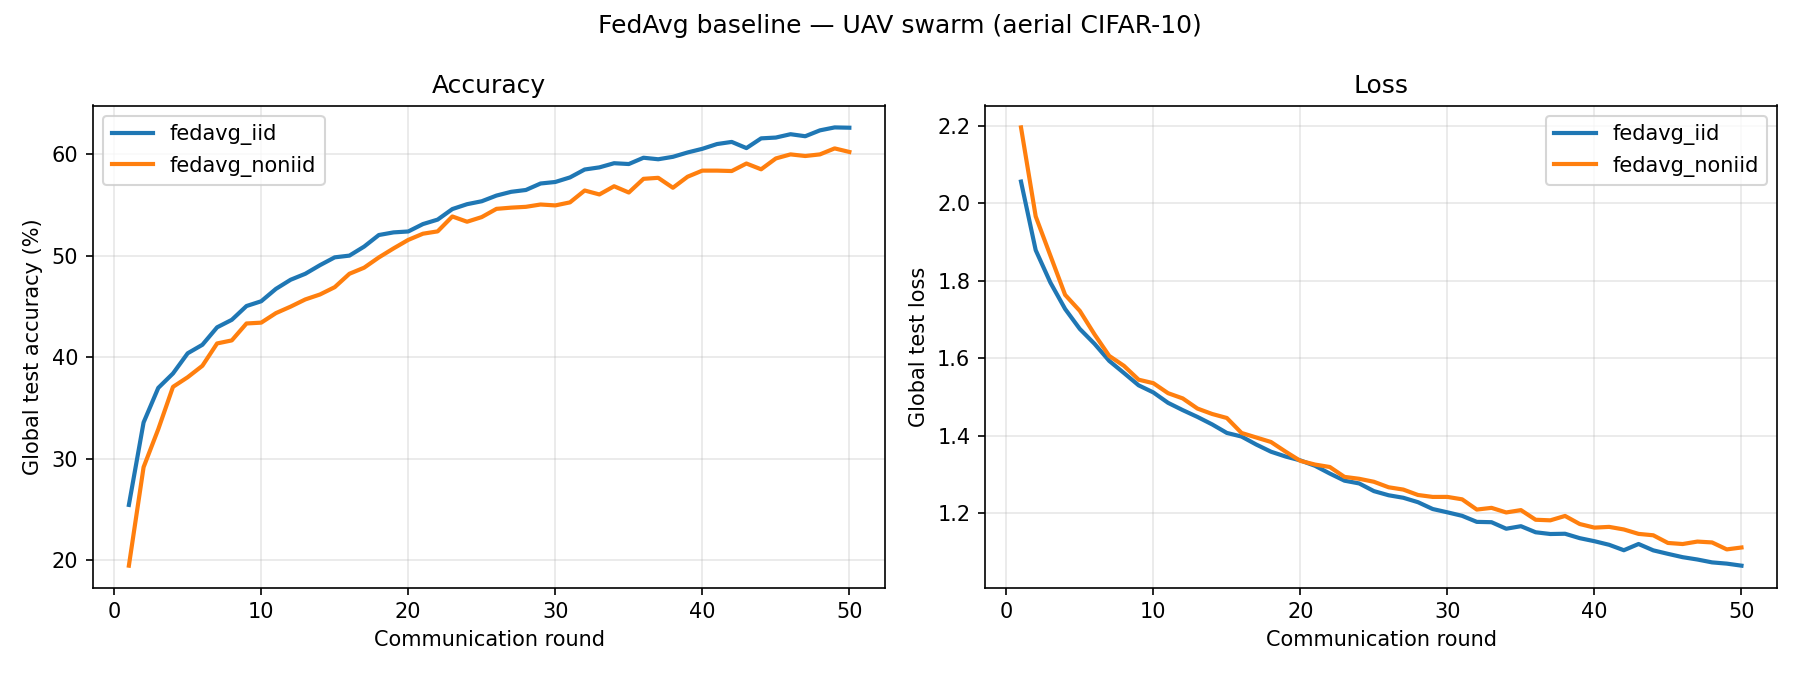
\includegraphics[width=\textwidth]{baseline_curves.png}
\caption{Test accuracy and loss of the FedAvg baseline over 50 rounds.}
\label{fig:baseline}
\end{figure}

Non-IID data cost about 2.4 percentage points, and neither curve had fully levelled
off by round 50. These numbers set the reference for the attack experiments: any
defence should keep accuracy close to them when no attack is present.

\section{Preliminary Study}
The preliminary study compared FedAvg, CosAvg and an early version of CCRA with one
BS, 30 rounds, one local epoch and a single seed. Three of the ten UAVs flipped their
labels, and in the jammed scenarios a ground jammer targeted three honest UAVs.
Table~\ref{tab:prelim} lists the final accuracy (mean of the last five rounds), and
Figs.~\ref{fig:prelim-acc} and~\ref{fig:prelim-weight} show the accuracy and the
weight each method gave to the attackers.

\begin{table}[ht]
\centering
\caption{Preliminary study: final accuracy (\%), single seed, 30 rounds}
\label{tab:prelim}
\begin{tabular}{@{}lccc@{}}
\toprule
Scenario & FedAvg & CosAvg & CCRA (early) \\
\midrule
No attack, ideal channel & 46.5 & \textbf{47.1} & 44.5 \\
No attack, jammed lossy channel & 44.6 & \textbf{45.6} & 43.1 \\
30\% label flip, ideal channel & 37.6 & 36.6 & \textbf{43.3} \\
30\% label flip, jammed lossy channel & 36.8 & 39.7 & \textbf{43.0} \\
\bottomrule
\end{tabular}
\end{table}

\begin{figure}[ht]
\centering
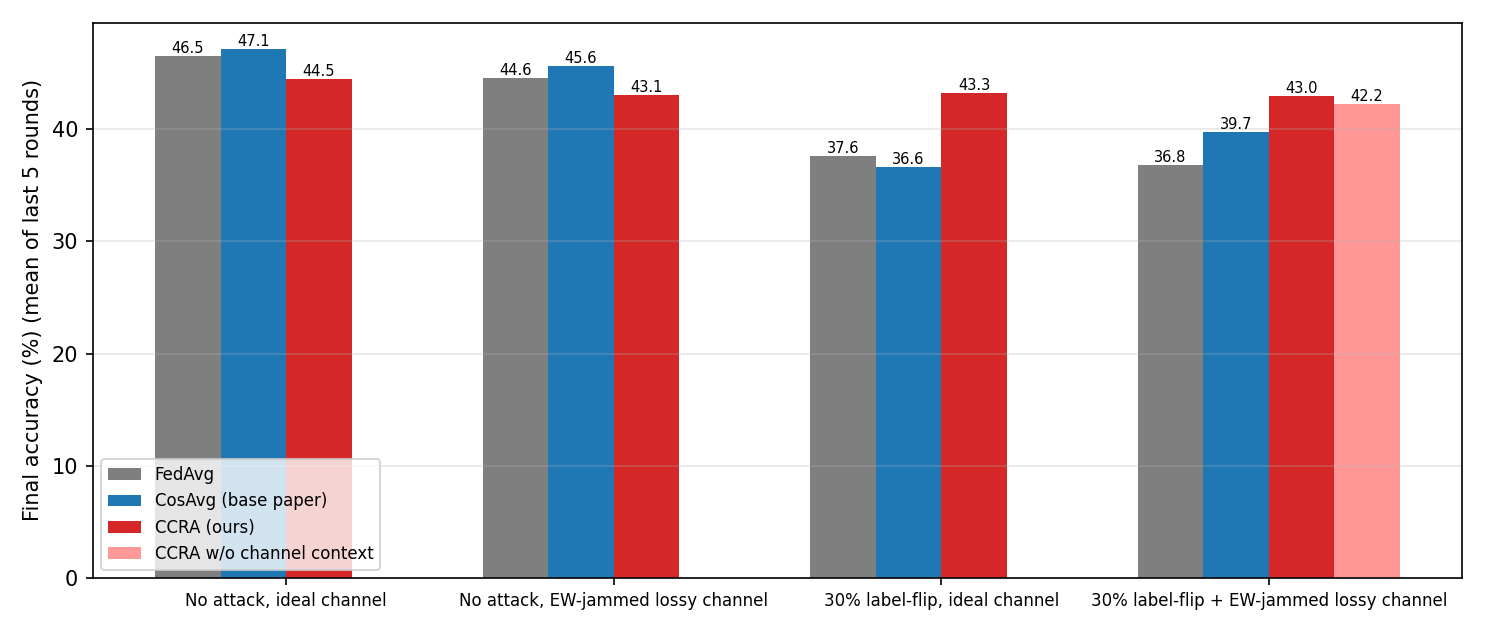
\includegraphics[width=\textwidth]{prelim_accuracy_bars.png}
\caption{Preliminary study: final accuracy in the four scenarios.}
\label{fig:prelim-acc}
\end{figure}

\begin{figure}[ht]
\centering
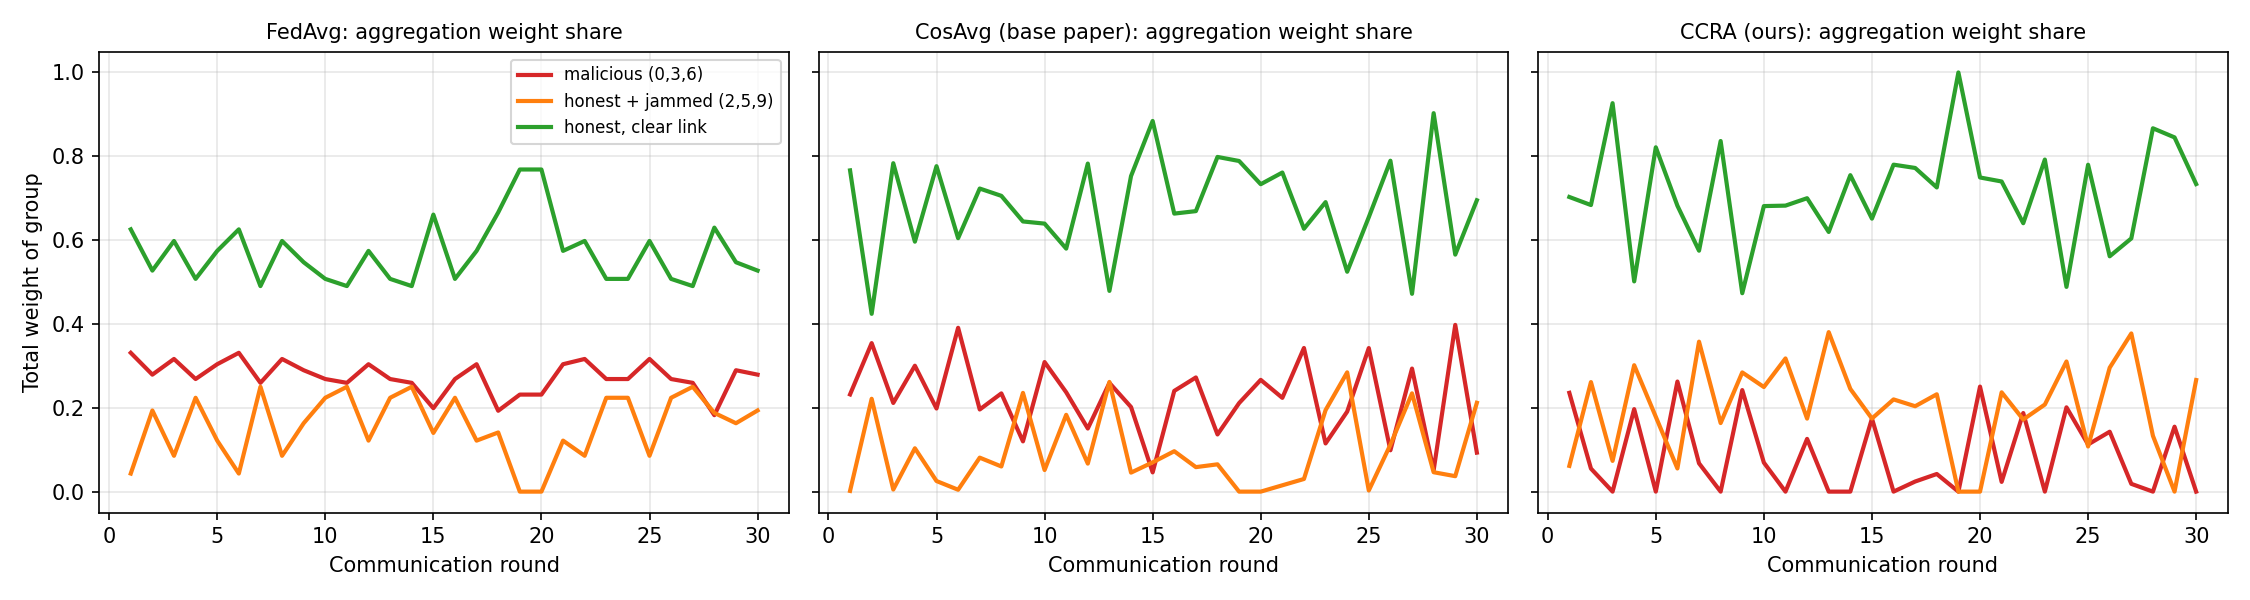
\includegraphics[width=0.9\textwidth]{prelim_weight_share.png}
\caption{Preliminary study: aggregation weight given to attackers and to jammed
honest UAVs under label flipping on the jammed channel.}
\label{fig:prelim-weight}
\end{figure}

The early CCRA kept about 43\% accuracy in every attacked scenario and gave the
attackers 1.9\% of the aggregation weight on the ideal channel, against 19.1\% for
CosAvg and 26.0\% for FedAvg. It cost about 2.5 points when there was no attack.
These results were encouraging, but they could not support a claim:
\begin{itemize}
\item they came from one seed, so the size of the random variation was unknown;
\item the channel-aware part of CCRA added only 0.8 points over its no-context
  ablation (42.2 to 43.0\%), well within single-run noise;
\item CCRA used a trusted root set while CosAvg did not, so the comparison mixed two
  differences;
\item the reputation rule was revised when the system was extended to hierarchical
  FL, so the early CCRA is not the exact version evaluated in the controlled study.
\end{itemize}
These limitations defined the controlled study.

\section{Controlled Ablation Study}
\label{sec:controlled}
All \NumRuns{} runs finished and were validated. The trace delivered on average
\PdrTrace\% of packets at 15\,dB and \PdrStress\% at 5\,dB.

\subsection{Stability and Overall Accuracy}
Table~\ref{tab:outcomes} summarizes every run, and Fig.~\ref{fig:acc} shows accuracy
under attack across the three channel conditions.

\begin{table}[ht]
\centering
\caption{Outcomes over all \NumRuns{} runs (120 per method). Diverged runs count as 10\%.}
\label{tab:outcomes}
\begin{tabular}{@{}lccc@{}}
\toprule
Method & Diverged & All runs (\%) & Attacked, 5\,dB (\%) \\
\midrule
FedAvg & 41/120 & 37.3 & 29.4 \\
Median & 26/120 & 29.3 & 21.3 \\
FLTrust & 0/120 & 50.6 & \textbf{50.1} \\
No-context & 0/120 & 51.4 & 45.3 \\
Mask-only & 0/120 & \textbf{52.8} & 49.5 \\
CCRA (full) & 0/120 & 51.1 & 46.0 \\
\bottomrule
\end{tabular}

\end{table}

\begin{figure}[ht]
\centering
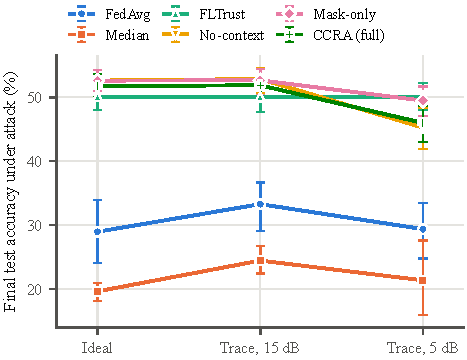
\includegraphics[width=0.75\textwidth]{accuracy_vs_channel.pdf}
\caption{Final accuracy under attack (mean over sign flip, ALIE and IPM and
\NumSeeds{} seeds), with 95\% bootstrap confidence intervals.}
\label{fig:acc}
\end{figure}

FedAvg diverged in \DivFedavg{} and the coordinate-wise median in \DivMedian{} of
their 120 runs; the sign-flip attack destroys FedAvg in every seed. None of the
methods that use a trusted reference update (FLTrust and the three CCRA variants)
diverged in any run. The median does worse than expected because each cell holds
only a few UAVs, so one attacker in a cell is already a large fraction of the values
being compared. Over all runs the mask-only variant has the highest accuracy,
\AllMask\%, against \AllFedavg\% for FedAvg. Table~\ref{tab:per-attack} breaks the
result down by attack.

\begin{table}[ht]
\centering
\caption{Mean final accuracy (\%) by attack, method and channel. Best value in each
block and column in bold.}
\label{tab:per-attack}
\small
\begin{tabular}{@{}llccc@{}}
\toprule
Attack & Method & Ideal & Trace, 15 dB & Trace, 5 dB \\
\midrule
No attack & FedAvg & \textbf{59.2} & \textbf{59.3} & 54.1 \\
 & Median & 52.5 & 52.7 & 49.7 \\
 & FLTrust & 52.5 & 51.5 & 52.9 \\
 & No-context & 57.1 & 56.7 & 51.1 \\
 & Mask-only & 57.1 & 57.5 & \textbf{54.7} \\
 & CCRA (full) & 55.4 & 56.6 & 52.6 \\
\midrule
Sign flip & FedAvg & 10.0 & 10.0 & 10.0 \\
 & Median & 10.0 & 19.6 & 12.4 \\
 & FLTrust & 50.0 & 49.9 & \textbf{50.6} \\
 & No-context & \textbf{54.2} & \textbf{53.8} & 46.1 \\
 & Mask-only & 54.2 & 53.6 & 49.9 \\
 & CCRA (full) & 52.5 & 52.8 & 46.5 \\
\midrule
ALIE & FedAvg & 49.8 & 46.9 & 42.0 \\
 & Median & 35.4 & 28.4 & 28.1 \\
 & FLTrust & 49.9 & 50.6 & 49.6 \\
 & No-context & \textbf{52.9} & 52.6 & 46.0 \\
 & Mask-only & 52.9 & \textbf{52.7} & \textbf{50.8} \\
 & CCRA (full) & 52.8 & 51.9 & 46.9 \\
\midrule
IPM & FedAvg & 27.0 & 42.9 & 36.0 \\
 & Median & 13.4 & 25.3 & 23.5 \\
 & FLTrust & 50.5 & 49.7 & \textbf{50.0} \\
 & No-context & \textbf{50.7} & \textbf{52.3} & 43.6 \\
 & Mask-only & 50.7 & 51.7 & 47.7 \\
 & CCRA (full) & 50.0 & 51.0 & 44.5 \\
\bottomrule
\end{tabular}

\end{table}

Two points in Table~\ref{tab:per-attack} deserve attention. First, with no attack,
plain FedAvg is the most accurate method on the ideal and 15\,dB channels; every
robust method pays a cost of roughly two to eight points for discarding or
down-weighting honest updates. Second, on the 5\,dB channel the masked variant is
slightly ahead of FedAvg even without an attack, consistent with FedAvg's zero-filled
lost coordinates now hurting it.

\subsection{Which Kind of Channel Awareness Helps}
Figure~\ref{fig:ablation} shows the paired contrasts that separate the two channel
mechanisms.

\begin{figure}[ht]
\centering
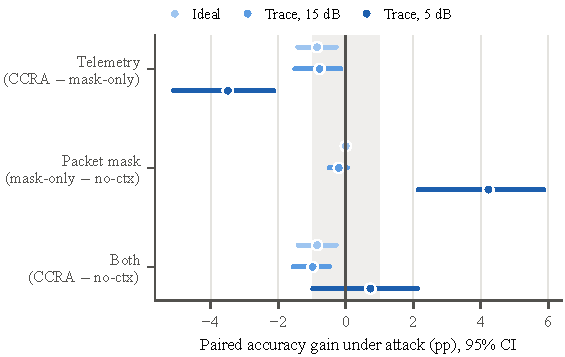
\includegraphics[width=0.75\textwidth]{ablation_contrasts.pdf}
\caption{Paired accuracy differences under attack with 95\% bootstrap intervals. The
grey band is the prespecified $\pm1$ point region of practical equivalence.}
\label{fig:ablation}
\end{figure}

\textbf{Erasure masking.} On the ideal channel nothing is lost, so mask-only and
no-context are identical. As the link weakens the masks matter more, and at 5\,dB
masking adds \MaskGain{} points (95\% CI \ci{\MaskLo}{\MaskHi}). Treating lost
coordinates as zeros shrinks honest updates, distorts their similarity scores and
pulls the average towards zero; ignoring them avoids all three effects.

\textbf{Telemetry in the reputation.} The prespecified primary estimate, the
telemetry effect at 5\,dB minus that at 15\,dB, is $\PrimGain$ points
(\ci{\PrimLo}{\PrimHi}). The whole interval lies below the $-1$ point threshold, so
by the rule fixed in advance the telemetry mechanism has a meaningful
\emph{negative} effect that grows as the link weakens. In absolute terms, at 5\,dB
CCRA minus mask-only is $\TelGain$ points (\ci{\TelLo}{\TelHi}): \AccCcraStress\%
against \AccMaskStress\%.

\textbf{Both together.} Full CCRA against no-context combines a gain and a loss; at
5\,dB the net effect is small and its interval includes the equivalence region. The
earlier impression that ``channel context helps'' came from this combination, which
hid two opposite effects.

\subsection{Mechanism: Who the Gate Rejects}
\label{sec:mechanism}
Section~\ref{sec:fixed-point} predicted that slowing rewards on weak links would push
honest UAVs' reputations down without doing much to attackers.
Figure~\ref{fig:gate} confirms that pattern.

\begin{figure}[ht]
\centering
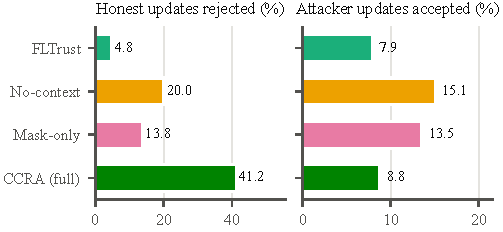
\includegraphics[width=0.75\textwidth]{gate_rates.pdf}
\caption{Gate decisions under attack at 5\,dB, as a percentage of received updates,
averaged over attacks and seeds.}
\label{fig:gate}
\end{figure}

With telemetry, the gate rejected \RejCcra\% of honest updates against \RejMask\%
without it, while the share of attacker updates accepted fell only from \AccptMask\%
to \AccptCcra\%. The rule gave up a large amount of honest data to filter slightly
more attacker data, and it did so precisely when honest data were already scarce
because of packet loss. These rates are descriptive. They agree with the analysis in
Section~\ref{sec:fixed-point}, but they do not by themselves prove that it is the
cause.

\subsection{Comparison with FLTrust}
FLTrust is the closest established method, since it uses the same root set. Its gate
rejected only \RejFltrust\% of honest updates at 5\,dB, because it has no memory:
each round is judged on its own. In an exploratory paired comparison, mask-only was
\VsFltTrace{} points better than FLTrust under attack at 15\,dB
(\ci{\VsFltTraceLo}{\VsFltTraceHi}), but at 5\,dB the two were indistinguishable
($\VsFltStress$ points, \ci{\VsFltStressLo}{\VsFltStressHi}). The two methods differ
in more than memory, so this comparison cannot isolate its effect; one reading
consistent with the mechanism above is that reputation memory helps on good links and
stops helping on weak ones.

\section{Discussion}
\subsection{What the Results Show}
\begin{enumerate}
\item A trusted reference update is what keeps training stable: every method that
  used one avoided divergence, and every method that did not diverged in some runs.
\item Among channel-aware mechanisms, erasure masking is simple, costs nothing on a
  good channel (its 15\,dB contrast is inside the equivalence region) and helps
  substantially on a weak one.
\item The intuitive idea of letting link quality soften judgement backfired. The
  failure is structural: an asymmetric reputation update biases trust downwards for
  exactly the UAVs it was meant to protect.
\end{enumerate}

\subsection{Why a Negative Result Is Useful}
The preliminary study suggested that CCRA's channel context was its key ingredient.
Had that claim been carried forward, Phase~II would have been built on a component
that harms accuracy. The prespecified design, paired seeds and chance scoring of
diverged runs made it possible to reject the claim with confidence, and the
analysis in Section~\ref{sec:fixed-point} points to the specific rule that must
change.

\subsection{Threats to Validity}
\begin{itemize}
\item \textbf{Channel realism.} The trace comes from one measured BS; the other BSs
  are virtual, and the 5 and 15\,dB anchors are assumptions, not calibrated values.
  The runs contain few handovers, so no claim is made about high mobility.
\item \textbf{Scope of learning task.} One dataset, one model, ten UAVs and fixed
  attack strengths were used.
\item \textbf{Attacker model.} Telemetry is assumed authentic, and adaptive attacks on
  the reputation itself~\cite{liu2026evade} were not tested.
\item \textbf{Statistics.} Ten seeds give approximate intervals; secondary contrasts
  are not adjusted for multiple comparisons. Any revised rule must be tested on new
  seeds, not re-tuned on these ten.
\end{itemize}

\chapter{Summary and Conclusions}
\label{ch:conclusions}

\section{Summary of the Work}
This project built a simulation framework for federated learning over a UAV swarm
whose updates travel over lossy air-to-ground links and in which some UAVs are
Byzantine. The framework supports hierarchical aggregation at three base stations,
handover, packet erasures from a synthetic jammed channel or a measured UAV trace,
five attacks and eight aggregation rules, and is covered by automated tests. A FedAvg
baseline was established first. A reputation-based aggregator, CCRA, was then
designed with two forms of channel awareness, erasure masking and telemetry-weighted
reputation. After a promising but inconclusive single-seed study, a prespecified,
paired study of \NumRuns{} runs separated the two forms and measured each one's
effect. The results have been written up as a manuscript in IEEE letter format.

\section{Conclusions}
\begin{enumerate}
\item Non-IID data reduced FedAvg accuracy from 62.6\% to 60.2\% in the baseline,
  and a 30\% label-flip attack reduced it by about ten points in the preliminary
  study.
\item Aggregators that judge updates against a trusted reference update never
  diverged in \NumRuns{} runs, whereas FedAvg and the coordinate-wise median
  diverged in \DivFedavg{} and \DivMedian{} of 120 runs each.
\item Ignoring lost coordinates instead of treating them as zeros (erasure masking)
  improved accuracy under attack on a 5\,dB link by \MaskGain{} percentage points
  (95\% CI \ci{\MaskLo}{\MaskHi}).
\item Using link telemetry to slow reputation rewards had a meaningful negative
  effect: the prespecified primary estimate was $\PrimGain$ points
  (\ci{\PrimLo}{\PrimHi}), and the gate rejected \RejCcra\% of honest updates
  instead of \RejMask\%.
\item The likely cause is structural. With slowed rewards but full-rate penalties,
  the fixed-point condition~\eqref{eq:fixed-point} shows that an honest UAV's
  reputation settles towards its worst rounds rather than its average behaviour, and
  the measured gate decisions match this prediction.
\item On weak links, the best variant is statistically indistinguishable from
  FLTrust (an exploratory comparison), so its advantage over FLTrust appears only on
  ideal and moderate channels.
\end{enumerate}

\section{Scope for Future Work (Phase II)}
\begin{enumerate}
\item \textbf{Redesign the reward rule} so that weak links do not bias reputation
  downwards, for example by making the update symmetric in the evidence, or by
  normalizing each UAV's score against its own recent history, and freeze the rule
  before testing.
\item \textbf{Confirm on fresh seeds and conditions.} Evaluate the revised rule on
  new seeds and channel settings rather than the ten used here, so that tuning
  cannot inflate the result.
\item \textbf{Mobility and handover.} Use traces or mobility models with frequent
  handovers, and more base stations, to test whether telemetry helps when the
  dominant impairment is handover rather than fading.
\item \textbf{Stronger attackers.} Add adaptive attacks that target the reputation
  itself and attackers that spoof their link telemetry.
\item \textbf{Network-level simulation.} Replace the packet-error model with a
  network simulator such as NS-3 to capture medium access, retransmissions and
  latency.
\item \textbf{Generalization.} Repeat the key comparisons with another dataset, a
  larger model and a larger swarm, and submit the manuscript.
\end{enumerate}


% 1.6: appendices numbered in Roman capitals, before the references.
\appendix
\renewcommand{\thechapter}{\Roman{chapter}}
\chapter{Experimental Settings}
\label{app:settings}

\begin{table}[ht]
\centering
\caption{Settings of the controlled study}
\label{tab:settings}
\begin{tabularx}{\textwidth}{@{}l X@{}}
\toprule
Parameter & Value \\
\midrule
UAVs $K$, base stations $B$ & 10, 3 \\
Byzantine UAVs $f$ & 3, fixed per seed across all methods \\
Rounds; synchronization period $E$ & 100; 5 \\
Local training & 1 epoch, SGD, learning rate 0.01, momentum 0.9, batch 64, weight decay $5\times10^{-4}$ \\
Model & TacticalEdgeCNN, about 156k parameters, group normalization \\
Data & Aerial-transformed CIFAR-10, Dirichlet $\alpha=0.5$, 49{,}500 training images to UAVs \\
Root set $\mathcal{D}_0$ & 500 images (50 per class), disjoint from all UAV data \\
Reputation & $\beta=0.5$, gate $\tau=0.3$, initial trust 1 \\
Staleness discount & $\exp(-0.5\,\cdot\,\text{staleness})$; late updates dropped \\
Packets & $L=1024$ parameters, 32 bits per parameter \\
Packet errors & logistic, slope $a=1$, threshold $\gamma_{\mathrm{th}}=3$\,dB \\
Round deadline; bandwidth & 2\,s; 20\,MHz \\
Handover & 3\,dB hysteresis, 2-round time to trigger \\
Trace & DeepSense~6G Scenario~23, stride 5 samples per round, segments $\ge 200$ samples \\
Reference SNR $\bar\gamma$ & 15\,dB (good link), 5\,dB (weak link) \\
Attacks & sign flip $\lambda=5$; ALIE-style $z=1.5$; IPM $\epsilon=0.5$ \\
Seeds & 41--50 \\
\bottomrule
\end{tabularx}
\end{table}

\chapter{Reproducing the Results}
\label{app:repro}

All code, the run-level results and this report are in the repository
\url{https://github.com/sasank-555/uav-swarm-fl}.

\begin{table}[ht]
\centering
\caption{Repository layout}
\label{tab:repo}
\begin{tabularx}{\textwidth}{@{}l X@{}}
\toprule
Path & Contents \\
\midrule
\texttt{fl/} & Simulator: data, model, client, channel, topology, attacks, aggregators, server \\
\texttt{tests/} & 43 automated tests \\
\texttt{run\_context\_study.py} & Plans and runs the \NumRuns-run controlled study \\
\texttt{analyze\_context\_study.py} & Prespecified analysis with paired bootstrap \\
\texttt{results/context\_study/} & Run-level CSV and analysis of the controlled study \\
\texttt{scripts/make\_paper\_figures.py} & Builds every figure, table and number in the paper and this report \\
\texttt{paper/} & Manuscript in IEEE letter format \\
\texttt{report/} & This report \\
\bottomrule
\end{tabularx}
\end{table}

The main steps are:
\begin{enumerate}
\item Install the dependencies: \texttt{pip install -r requirements.txt}.
\item Prepare the data: \texttt{python prepare\_data.py}, and convert the DeepSense
  Scenario~23 download with \texttt{scripts/prepare\_deepsense23.py}.
\item Run the study (about 720 GPU runs):
  \texttt{python run\_context\_study.py --profile final --device cuda --parallel 4}.
\item Analyse it: \texttt{python analyze\_context\_study.py results/context\_final}.
\item Rebuild all figures and numbers: \texttt{python scripts/make\_paper\_figures.py}.
\end{enumerate}
Step~5 alone is enough to regenerate this report's figures from the committed results.


% 1.7: literature cited, IEEE style.
\bibliographystyle{IEEEtran}
\bibliography{refs}

% 1.8-1.9: publications, then acknowledgements.
% 1.8: publications by the candidates on the topic of the project.
\chapter*{Publications}
\addcontentsline{toc}{chapter}{Publications}

\begin{enumerate}[label={[P\arabic*]}, leftmargin=12mm]
\item \textit{Erasure-Aware Byzantine-Robust Aggregation for Hierarchical UAV-Swarm
  Federated Learning: When Link Telemetry Hurts}, manuscript in preparation for an IEEE
  letters journal (IEEE Communications Letters, IEEE Wireless Communications Letters
  or IEEE Networking Letters).
\end{enumerate}

% 1.9: acknowledgements, after the references, signed and dated.
\chapter*{Acknowledgements}
\addcontentsline{toc}{chapter}{Acknowledgements}

We thank our supervisor, \Supervisor, for steering this project towards realistic
wireless conditions and fair, like-for-like comparisons, and for asking us to state
our findings with the evidence behind them. We thank the Head of the Department,
\HOD, and the faculty of the \Department{} for their support. We also thank the
creators of the DeepSense~6G dataset for making their UAV measurements available.

\vspace{18mm}
\noindent
{\renewcommand{\Student}[2]{%
  \begin{minipage}[t]{0.32\textwidth}\centering
  \rule{40mm}{0.4pt}\\#1\\#2
  \end{minipage}\hfill}%
\StudentList}

\vspace{10mm}
\noindent Date: \rule{40mm}{0.4pt}


\end{document}
